\chapter{Background}
\label{cha:background}

\section{Cellular automata}

\Acp{CA} were originally proposed by Stanislaw Ulam and John Von
Neumann in the 1940s as a model of the growth of crystals and an attempt at
constructing a self-replicating system \cite{von_neumann_theory_1966}.

It is usually defined on a regular lattice in one or two dimension. Each of its
components is called a cell, and can be in a state $k \in \mathcal{S}$. A neighborhood
function $\boldsymbol{N}$ is defined which associates each cell with its
neighbors on the lattice.

In general, a \ac{CA} can be constructed on any space
$\mathcal{L}$ where such a function can be defined.
In practice, regular finite or infinite grids are chosen, $\mathcal{L} \subset \mathbb{Z}$ or
$\mathcal{L} \subset \mathbb{Z}^{2}$. For example, the grid could be a 1-dimensional torus with 10 cells,
that is $\mathcal{L}_{{T_{10}}} = \{1, 2, \ldots, 10 \}$.

The neighborhood function has the form

\begin{equation}
  \begin{aligned}
\boldsymbol{N} :\quad & \mathcal{L} \rightarrow \mathcal{L}^{s}\\
&c \mapsto [c_{i}]_{i=1}^{s}
  \end{aligned}
\end{equation}
,

where the returned value is a finite number of cells, the neighbors of cell $c$.
For the torus $\mathcal{L}_{T_{10}}$ above, we can define the neighbors to be the cell
itself and the two immediately adjacent cells. This type of 1D neighborhood is
illustrated on Figure \ref{fig:1d_neigh}. It corresponds to the following
neighborhood function
\begin{equation}
  \begin{aligned}
\boldsymbol{N} :\quad & \mathcal{L}_{T_{10}} \rightarrow \mathcal{L}_{T_{10}}^{3} \\
&\boldsymbol{N}(c) = \begin{cases}
                      [c - 1, c, c + 1],& \text{if}\quad c \in \{2,\ldots , 9\}\\
                       [10, 1, 2], & \text{if} \quad c = 1 \\
                       [9, 10, 1], & \text{if} \quad c = 10. \\
                    \end{cases}
  \end{aligned}
\end{equation}

On two dimensional grids, there are multiple ways to define the neighborhood.
Some common examples are the Moore neighborhood and the Von Neumann neighborhood.

\begin{figure}[htbp]
  \centering
  \begin{subfigure}[c]{.3\linewidth}
    \centering
    
\includegraphics[width=\linewidth]{figures/1d_neigh}
    \caption{Standard 1D \ac{CA} neighborhood}
    \label{fig:1d_neigh}
  \end{subfigure}
  \begin{subfigure}[c]{.3\linewidth}
    \centering
    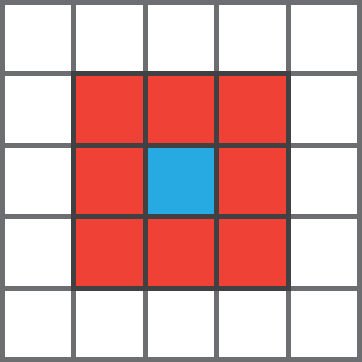
\includegraphics[width=\linewidth]{figures/moore}
    \caption{Moore neighborhood}
    \label{fig:moore}
  \end{subfigure}
  \begin{subfigure}[c]{.3\linewidth}
    \centering
    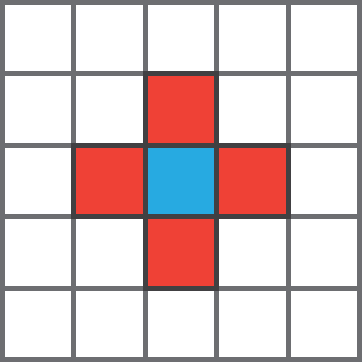
\includegraphics[width=\linewidth]{figures/von_neumann}
    \caption{Von Neumann neighborhood}
    \label{fig:von_neumann}
  \end{subfigure}

  \caption{Illustration of commonly used neighborhoods for 1D and 2D cellular automata.}
  \label{fig:neighborhoods}
\end{figure}


An update rule $\boldsymbol{\Phi}$ defines the new state of a cell as a function of its local
neighborhood. It is applied in parallel to all the cells.

A large number of variants of \acp{CA} have been constructed. We list some of
them here.

\subsection{Asynchronous cellular automata}
A cellular automaton is said to be asynchronous when its cells are not all
updated in parallel at each time step.

\subsection{Stochastic cellular automata}
A cellular automaton is said to be asynchronous when its cells are not all
updated in parallel at each time step.

\subsection{Discrete}
\subsection{Continuous}

\section{Reservoir computing}
